% paper.tex — arXiv submission driver for the r_3(212) campaign writeup.
%
% Build:
%   latexmk -pdf paper.tex
% or:
%   pdflatex paper.tex && bibtex paper && pdflatex paper.tex && pdflatex paper.tex
%
% Source structure:
%   paper.tex          — this driver: preamble, title, abstract, \input{}'s
%   paper.body.tex     — generated by pandoc from sections-concatenated.md
%   refs.bib           — bibliography (see refs.bib)
%   anc/               — arXiv ancillary files (JSONL benchmarks, Lean encoding)

\documentclass[11pt,reqno]{amsart}

% --- Math and symbols ---
\usepackage[utf8]{inputenc}
\usepackage{amsmath,amssymb,amsthm,mathtools}
% \usepackage{stmaryrd}  % unused (no \llbracket in body)      % for \llbracket \rrbracket
% Keep the arXiv driver pdflatex-friendly. The pandoc body pass should convert
% unicode math symbols to LaTeX macros before final build.
% \usepackage{unicode-math}
\DeclareUnicodeCharacter{00A7}{\S}
\DeclareUnicodeCharacter{00B7}{\ensuremath{\cdot}}
\DeclareUnicodeCharacter{00D7}{\ensuremath{\times}}
\DeclareUnicodeCharacter{2026}{\dots}
\DeclareUnicodeCharacter{2192}{\ensuremath{\to}}
\DeclareUnicodeCharacter{21A6}{\ensuremath{\mapsto}}
\DeclareUnicodeCharacter{2208}{\ensuremath{\in}}
\DeclareUnicodeCharacter{2212}{-}
\DeclareUnicodeCharacter{2216}{\ensuremath{\setminus}}
\DeclareUnicodeCharacter{2227}{\ensuremath{\wedge}}
\DeclareUnicodeCharacter{2264}{\ensuremath{\leq}}
\DeclareUnicodeCharacter{2265}{\ensuremath{\geq}}
\DeclareUnicodeCharacter{2282}{\ensuremath{\subset}}
\DeclareUnicodeCharacter{2286}{\ensuremath{\subseteq}}

% --- Typography and layout ---
\usepackage[T1]{fontenc}
\usepackage{lmodern}
\usepackage{microtype}
\usepackage[margin=1in]{geometry}
\usepackage{parskip}

% --- Tables and floats ---
\usepackage{booktabs}      % for \toprule \midrule \bottomrule
\usepackage{array}
\usepackage{tabularx}
\usepackage{longtable}     % pandoc may emit longtable
\usepackage{float}
\newcounter{none}          % Pandoc uses LTcaptype=none for uncaptioned tables.

% --- Figures and algorithms ---
\usepackage{graphicx}
\usepackage{tikz}
\usetikzlibrary{positioning,arrows.meta,fit}
% \usepackage{algorithm}    % unused
% \usepackage{algpseudocode} % unused

% --- Cross-references ---
\usepackage[colorlinks=true,linkcolor=blue,citecolor=blue,urlcolor=blue]{hyperref}
\usepackage{cleveref}

% --- Code listings (for SAT/CDCL configs etc.) ---
\usepackage{listings}
\lstset{
  basicstyle=\ttfamily\small,
  breaklines=true,
  columns=fullflexible,
  keepspaces=true,
  frame=single,
  framerule=0.4pt,
  xleftmargin=0.5em,
}

% Pandoc emits this command for compact lists.
\providecommand{\tightlist}{%
  \setlength{\itemsep}{0pt}\setlength{\parskip}{0pt}}

% --- Theorem environments ---
\newtheorem{theorem}{Theorem}[section]
\newtheorem{lemma}[theorem]{Lemma}
\newtheorem{proposition}[theorem]{Proposition}
\newtheorem{corollary}[theorem]{Corollary}
\theoremstyle{definition}
\newtheorem{definition}[theorem]{Definition}
\newtheorem{problem}[theorem]{Problem}
\newtheorem{conjecture}[theorem]{Conjecture}
\theoremstyle{remark}
\newtheorem{remark}[theorem]{Remark}

% --- Macros ---
\newcommand{\Nset}{\mathbb{N}}
\newcommand{\Zset}{\mathbb{Z}}
\DeclareMathOperator{\rsymb}{r}
\newcommand{\rthree}[1]{\rsymb_{3}(#1)}
\newcommand{\Tone}{\ensuremath{\mathsf{T1}}}
\newcommand{\Tonea}{\ensuremath{\mathsf{T1a}}}
\newcommand{\Toneb}{\ensuremath{\mathsf{T1b}}}
\newcommand{\Tonec}{\ensuremath{\mathsf{T1c}}}
\newcommand{\Ttwo}{\ensuremath{\mathsf{T2}}}
\newcommand{\Tthree}{\ensuremath{\mathsf{T3}}}

% --- Frontmatter ---
\title[A Salem--Spencer solver benchmark]{Salem--Spencer sets as a
  cross-paradigm solver benchmark: a witness-split CP-SAT campaign on
  $\rthree{212}$ and a paradigm-resistant residual}

\author{Mehmet Ergezer}
\thanks{ORCID: \href{https://orcid.org/0000-0001-6627-3667}{0000-0001-6627-3667}.}
\address{Wentworth Institute of Technology, Boston, MA, USA}
\email{ergezerm@wit.edu}
% \author{Co-author Name}     % add as needed
% \address{Institution}
% \email{email}

\subjclass[2020]{
  Primary 11B25;
  Secondary 11Y16, 68W30, 68V20, 90C10
}

\keywords{
  constraint programming,
  benchmark instances,
  Salem--Spencer numbers,
  arithmetic progressions,
  OEIS A003002,
  CP-SAT,
  MIP,
  CDCL,
  DRAT proofs,
  formal verification,
  Lean
}

\date{July 3, 2026}

\begin{document}

\begin{abstract}
Deciding whether a $44$-element subset of $[1, 212]$ can avoid all
three-term arithmetic progressions is the current frontier instance of the
Salem--Spencer sequence $\rthree{N}$ (OEIS A003002) --- a family of finite
combinatorial feasibility problems that, unlike recent celebrated
SAT-solved problems in Ramsey-type combinatorics, resists every
off-the-shelf solver paradigm we tested. We present the problem family as
a constraint-solving benchmark. Our campaign architecture combines a
verified lower-bound witness, endpoint forcing, depth-$d$ witness-variable
splitting, window-cardinality inequalities derived from known $\rthree{L}$
values, and recursive refinement of timed-out subproblems. Applied to
$N = 212$, $K = 44$, it found no feasible $44$-set across millions of
CP-SAT subproblems, supporting but not proving the conjectured
$\rthree{212} = 43$. The window-cardinality family is the single most
effective pruning layer, reducing the unresolved rate by $28$ percentage
points. Cross-paradigm analysis of the resistant residual shows a sharp
stratification: an eight-hour HiGHS MIP audit closes $25$ of $45$
survivors while leaving $20$ with dual bounds pinned at $0.0$; pure CDCL
closes $18$ of those $20$, each with an independently verified DRAT proof;
and the final two subproblems (\Tonec) resist CP-SAT propagation, LP-based
MIP, and CDCL under generous wall caps. We release tiered benchmark
instances spanning this difficulty ladder, the verified DRAT/LRAT
certificates, a deterministic instance generator, and a Lean
formal-proof-search encoding of \Tonec, and frame the unit-gap problem
$\rthree{212} \in \{43, 44\}$ as a challenge for stronger inference,
custom branch-and-bound, or formal proof search.
\end{abstract}

\maketitle

% --- Body (generated by pandoc from sections-concatenated.md) ---
\section{Introduction and background}\label{introduction-and-background}

Let $r_3(N)$ denote the maximum size of a subset of $[1, N]$ containing no
nontrivial three-term arithmetic progression. Equivalently,

\[
  r_3(N) \;=\; \max\bigl\{\, |A| \;:\; A \subseteq [1, N],\
  \text{no } a < b < c \text{ in } A \text{ satisfy } a + c = 2b \,\bigr\}.
\]

The asymptotic study of $r_3(N)$ begins with Roth's theorem \cite{roth-1953}
and continues through Salem--Spencer and Behrend-type lower-bound
constructions \cite{salem-spencer-1942,behrend-1946} and modern
density-increment upper bounds, including work of Bloom--Sisask and
Kelley--Meka \cite{bloom-sisask-2023,kelley-meka-2023}. Those results
describe the large-$N$ behavior of progression-free sets. The present paper is
about a different but complementary problem: exact finite computation at the
OEIS A003002 frontier.

OEIS A003002 tabulates exact values of $r_3(N)$. Cariboni's b-file currently
reaches $N = 211$, where $r_3(211) = 43$
\cite{oeis-a003002,cariboni-b003002}. The next natural decision problem is
therefore:

\begin{quote}
Does there exist a 44-element 3-AP-free subset of $[1, 212]$?
\end{quote}

We found and independently verified a 43-element 3-AP-free subset of
$[1, 212]$, so the lower bound $r_3(212) \geq 43$ is settled. The upper-bound
question is whether $r_3(212) \leq 43$. Since $r_3(211) = 43$, any hypothetical
44-set in $[1, 212]$ must contain both endpoints 1 and 212; otherwise it
would translate or restrict to a 44-set in $[1, 211]$. Thus the target is a
single finite feasibility problem with a strong necessary endpoint condition.

Finite feasibility problems of this Ramsey-combinatorial flavor have been a
showcase for modern SAT and constraint solving: the Boolean Pythagorean
triples problem \cite{heule-kullmann-marek-2016}, Schur number five
\cite{heule-2018-schur}, and Keller's conjecture in dimension seven
\cite{brakensiek-heule-2020-keller} were each closed by massively parallel
CDCL search with machine-checkable proofs. The Salem--Spencer family sits in
the same problem class --- Boolean variables, one short linear constraint per
arithmetic progression, a cardinality target --- and, as this paper
documents, it separates tested solver configurations unusually sharply.
None of six monolithic CP-SAT, HiGHS, or CaDiCaL configurations resolves
the frontier instance in 24 hours. Under a witness-informed split, CP-SAT
and HiGHS leave a common residual pocket, while CDCL closes it --- but
implementation-dependently: the two hardest audited subproblems defeat the
tested CaDiCaL configuration at a 12-hour wall yet fall to kissat well
within that budget, with independently verified DRAT certificates.
That layered separation is precisely what makes the family interesting as
a benchmark: it is natural, scalable in $N$, has verifiable ground truth
at solved sizes, and grades solvers along a measured difficulty ladder
rather than a single pass/fail line.

We attacked this feasibility problem computationally using a reproducible
CP-SAT architecture. The model uses Boolean variables $x_i$, one linear
constraint for each 3-term arithmetic progression, the decision equality
$\sum_i x_i = 44$, endpoint forcing, reflection symmetry breaking, and
window-cardinality inequalities derived from the known values of $r_3(L)$ for
$L \leq 211$. To make the search tractable, we split the problem by assigning
high-degree variables from a verified 43-witness, generating a deterministic
depth-24 chunk space, and then refine residual \texttt{UNKNOWN} chunks recursively.

The campaign did not produce a formal proof of $r_3(212) = 43$. It did produce
four concrete outcomes.

First, we observed zero feasible 44-sets across millions of CP-SAT
subproblems, including broad chunks, recursive refinements, wall-cap
recalibrations, and targeted A/B experiments. This is empirical evidence for
the expected value $r_3(212) = 43$, but it is not a certificate.

Second, we found that OEIS window-cardinality inequalities are essential. On
controlled broad-pass ranges, adding these inequalities reduced the \texttt{UNKNOWN}
rate by roughly 28 percentage points and also reduced aggregate solver time.
They are the main successful pruning layer of the campaign.

Third, we identified and stratified a structural hard pocket. The
largest retained broad run over 100,000 depth-24 chunks left 6,071
\texttt{UNKNOWN} chunks. A uniform random 100-chunk sample of those 6,071
(seed 5230)
was passed through a 300-second recap, leaving 45 resistant survivors.
Re-attacking those 45 chunks with HiGHS, an
LP-relaxation-based MIP solver, closed 0/45 in one-hour-per-chunk runs.
A full eight-hour audit later closed 25/45, but left 20/45
\texttt{UNKNOWN}. A subsequent pure CDCL/SAT attack (CaDiCaL via PySAT)
closed 18/20 of that CP-SAT/HiGHS-resistant subset,
while two chunks --- T1c --- remained \texttt{UNKNOWN} even under a 12-hour
pure-CDCL cap and a 4-hour windowed-CDCL diagnostic.

Fourth, the pocket collapses under a current competition-grade CDCL
solver. Kissat 4.0.4 refutes both T1c chunks on the pure
3-AP/cardinality encoding, well within the budget under which CaDiCaL
failed, and both refutations are certified end-to-end: \texttt{drat-trim}
independently verified the DRAT proofs against sha256-pinned formula
files (§4.4). A kissat survey over a fresh uniform 100-chunk sample
of the broad residual closes 99/100 within a 2-hour cap. In the tested
configurations, the obstruction that survived CP-SAT tuning, HiGHS, and
CaDiCaL is therefore not intrinsic to the problem family: it is sensitive
to solver implementation and configuration. The pipeline isolates and
archives the instances on which those configurations diverge.

This paper's contribution is the benchmark and the cross-solver empirical
study, not a new exact value of A003002. We provide:

\begin{enumerate}
\def\labelenumi{\arabic{enumi}.}
\tightlist
\item
  A tiered benchmark release spanning a measured difficulty ladder: the
  25 HiGHS-closable T1a chunks, the 18 CaDiCaL-closable
  T1b-minus-T1c chunks, the 2 T1c chunks that separate CaDiCaL from
  kissat, the 6,071 broad \texttt{UNKNOWN} chunks from the 100k
  expansion batch, and a deterministic generator for the full
  depth-24 sweep.
\item
  A characterization of the structural hard pocket across CP-SAT, HiGHS,
  and two CDCL configurations. The pocket that initially appeared robust
  across formulations is closed outright by kissat 4.0.4, showing that the
  measured boundary is implementation- and configuration-sensitive.
\item
  A reproducible witness-split plus window-cardinality architecture for
  exact $r_3(N)$ upper-bound search, parametric in $(N, K)$
  and reusable at adjacent frontier sizes. The problem-specific
  window-cardinality inequalities are, empirically, worth more than any
  generic solver lever we tested.
\item
  A detailed empirical account of the $N = 212$, $K = 44$ campaign, including
  broad-pass counts, refinement behavior, solver-time tradeoffs, and the
  controlled A/B experiments behind each design decision.
\end{enumerate}

For reference, the benchmark tier notation used throughout the paper is:

{\def\LTcaptype{none} % do not increment counter
\begin{longtable}[]{@{}l
  >{\raggedright\arraybackslash}p{(\linewidth - 4\tabcolsep) * \real{0.8000}}@{}}
\toprule\noalign{}
Symbol & Meaning \\
\midrule\noalign{}
\endhead
\bottomrule\noalign{}
\endlastfoot
T1 & the 45 chunks that survived the 300-s recap of a random 100-chunk sample from the 6,071 broad UNKNOWNs \\
T1a & the 25 T1 chunks closed by the full 8-h HiGHS audit \\
T1b & the 20 T1 chunks left UNKNOWN by the full 8-h HiGHS audit \\
$\mathrm{T1b}\setminus\mathrm{T1c}$ & the 18 T1b chunks closed by CDCL and independently verified by DRAT checking \\
T1c & the final two chunks $\{40959, 48895\}$: resist CP-SAT, HiGHS, and CaDiCaL; refuted by kissat 4.0.4 with verified DRAT proofs \\
T2 & the 6,071 UNKNOWN chunks from the 100k broad expansion batch \\
T3 & the full 12,582,912-chunk AP-pruned depth-24 sweep \\
\end{longtable}
}

\subsection{Related work}\label{related-work}

\textbf{Split-and-solve search.} The witness-split architecture of §2.2
belongs to the cube-and-conquer family
\cite{heule-kullmann-wieringa-biere-2012}: partition the search space by
fixing a prefix of variable assignments (cubes), then solve each cube with
a complete solver. The differences are the cube-selection policy and the
refinement loop. Classical cube-and-conquer selects split variables by
lookahead heuristics; we select them by AP-incidence degree \emph{within a
verified extremal witness}, exploiting the problem-specific intuition that
a hypothetical 44-set must interact heavily with the densest
regions of the known 43-set. Timed-out cubes are then re-split
recursively (§2.4), which parallels iterative cube deepening.

\textbf{Implied constraints and streamliners.} The window-cardinality
inequalities of §2.3 are implied constraints in the standard CP-modeling
sense: they are logical consequences of the base 3-AP model that are not
explicitly present and are not efficiently recovered by the tested
propagators. They are derived from previously \emph{computed} values of the
same sequence --- the solved prefix of A003002 prunes the frontier
instance. This is soundness-preserving, in contrast to streamlined
constraint reasoning \cite{gomes-sellmann-2004}, which deliberately
sacrifices completeness; it is closer in spirit to bound propagation from
tabulated subproblem optima. Empirically these inequalities dominate
every generic lever we tested (§3.3, §4.5).

\textbf{SAT and CP in combinatorial mathematics.} Beyond the celebrated
results cited above, exact computation of Salem--Spencer values has its
own lineage: Dybizba\'nski \cite{dybizbanski-2012} computed
$r_3(N)$ through $N = 123$ with a tailored
branch-and-bound, and Cariboni's OEIS b-file \cite{cariboni-b003002}
extends the sequence to $N = 211$. Our campaign differs in
attacking the frontier with general-purpose solvers plus
problem-specific pruning, and in reporting the negative space --- which
subproblems resist and why --- rather than only the closed values.

\textbf{Benchmarks and certified solving.} Curated instance families ---
CSPLib \cite{gent-walsh-1999-csplib}, MIPLIB \cite{gleixner-miplib-2021},
the SAT Competition suites --- have repeatedly steered solver research
toward documented failure modes. The tiered release of §5 is offered in
that tradition: a natural family, scalable in $N$, with verifiable
ground truth at solved sizes and a measured cross-solver difficulty
ladder. On the certification side, the CDCL-closed tier ships with
DRAT proofs verified by \texttt{drat-trim}
\cite{heule-hunt-biere-drat-2014,cruz-filipe-lrat-2017}; the absence of
comparable certificates for the CP-SAT and MIP closures (§6.2) is an
instance of the gap that auditable constraint solving
\cite{gocht-mccreesh-nordstrom-2022} aims to close.

\subsection{Organization}\label{organization}

The rest of the paper is organized as follows. §2 describes the
architecture. §3 reports the computational campaign, beginning with the
monolithic baseline. §4 analyzes the hard pocket across HiGHS, CaDiCaL,
and kissat, ending in its collapse and the refutation of our working
hypothesis. §5 releases the tiered benchmark and estimates the remaining
path to a full certificate. §6 discusses transferability, limitations,
and what the campaign suggests about finite $r_3$ upper-bound search.

\section{Architecture}\label{architecture}

The campaign rests on five components: a decision-form CP-SAT model
of the 3-AP-free subset problem (§2.1), a witness-variable splitting
scheme that produces tractable subproblems (§2.2), a window-cardinality
pruning family derived from OEIS A003002 (§2.3), a recursive refinement
loop for residual \texttt{UNKNOWN} chunks (§2.4), and the SLURM-side
engineering that makes the workload reproducible (§2.5). Each
component is independent of the others --- any could be replaced by a
stronger variant without disturbing the rest --- and together they
define the proof attempt on $r_3(212) \leq 43$.

\subsection{Decision-form CP-SAT model}\label{decision-form-cp-sat-model}

Fix $N \geq 3$ and $K \geq 3$. The standard CP-SAT encoding of ``does
there exist a 3-AP-free subset $A \subseteq [1,N]$ with $|A| \geq K$?''
introduces Boolean variables $x_i \in \{0,1\}$ for $i \in [1,N]$, with
$x_i=1$ if and only if $i \in A$, and adds
\[
  x_a+x_b+x_c \leq 2
  \quad\text{for every 3-AP triple }(a,b,c),
  \qquad
  \sum_{i=1}^{N}x_i \geq K.
\]

We adopt the \textbf{decision-form} variant in which the second inequality
is replaced by the equality

\[
  \sum_{i=1}^{N}x_i = K.
\]

The decision-form encoding is tighter for propagation, not for logical
interpretation of \texttt{UNKNOWN}: an \texttt{UNKNOWN} return on either encoding is still
consistent with both feasibility and infeasibility. The practical advantage of
$\sum_i x_i = K$ is that CP-SAT and pseudo-Boolean propagators see both the
lower and upper cardinality directions. Branches that would require more than
$K$ selected values, or too few remaining unfixed values to reach $K$, can be
cut earlier than in the inequality form. For our purposes (proving the upper
bound $r_3(N) \leq K-1$), the equality form is therefore the right primitive.

For $N = 212$, $K = 44$, the model has 212 Boolean variables and
11,130 3-AP triple inequalities. We add the lex symmetry-breaking
constraint

\[
  (x_1,x_2,\ldots,x_N) \geq_{\mathrm{lex}}
  (x_N,x_{N-1},\ldots,x_1).
\]

to factor out the reflection $i \mapsto N+1-i$. The opposite orientation would
be equivalent; the implementation uses the displayed orientation. We do not add other
symmetries. After endpoint forcing, reflection is the only order-preserving
symmetry we exploit.

We also apply \textbf{endpoint forcing} specific to the $r_3(212)$ case.
Since OEIS A003002 records $r_3(211) = 43$, any 44-element
3-AP-free subset of $[1, 212]$ must contain both endpoints 1
and 212: if 1 were absent, the set would be a 44-element
3-AP-free subset of $[2, 212]$, which shifts to $[1, 211]$; if 212
were absent, it would already lie in $[1, 211]$. Either case contradicts
$r_3(211) = 43$. We add $x_1=x_{212}=1$ as ground assumptions in
every chunk.

Branching: variable selection by AP-incidence degree (the number of
3-AP triples a variable appears in), value selection \texttt{min}, and
\texttt{fixed\_search} to disable CP-SAT's portfolio search. The first two
target the most-constrained variables first; the third reduces solver-policy
variation across runs, which is necessary for the A/B experiments of §3.3
and §3.6.

\subsection{Witness-variable splitting}\label{witness-variable-splitting}

The decision-form model on the full range $[1, 212]$ is already at
the limit of single-call CP-SAT solving in reasonable wall time. To
break it into tractable subproblems we use a cube-and-conquer-style split
\cite{heule-kullmann-wieringa-biere-2012} in which the cubes are chosen
not by lookahead but from the verified 43-element
lower-bound witness $A_{43} \subset [1,212]$ (§2.1, §3.2). The
splitting proceeds in three steps.

\textbf{Degree ranking.} For each $v \in A_{43}$, compute the AP-incidence
degree
\[
  \deg(v)=\bigl|\{(a,b,c):v\in\{a,b,c\},\ b-a=c-b\}\bigr|.
\]
Sort $A_{43}$ by $\deg(v)$ in decreasing order. Pick the top
$d = 24$ witness values; we refer to this prefix as the \textbf{broad split
prefix}.

\textbf{Combinatorial enumeration.} For each of the
$2^{24}=16{,}777{,}216$
IN/OUT assignments of the broad split prefix, instantiate a
\textbf{chunk}: the decision-form model with $x_v$ fixed to the chosen
value for every $v$ in the prefix. A chunk is identified by its
24-bit chunk ID.

\textbf{AP-prefix pruning.} Many chunks are immediately infeasible at the
3-AP level alone: if the broad split prefix forces three pinned-IN
values that form a 3-AP, the chunk has no feasible completion and
need not be sent to CP-SAT. We perform this check during chunk
emission and skip such chunks. The surviving chunk count for
$N = 212$, $K = 44$ at depth 24 is 12,582,912, roughly 75\% of
the raw $2^{24}$ count.

The choice $d = 24$ is empirical: larger $d$ produces more chunks but
each is easier; smaller $d$ produces fewer chunks but each is harder.
At $d = 24$ the per-chunk solver time at the 60-s wall cap has a
heavy tail but a tractable median (the broad pass closes approximately
94\% of expansion chunks within 60 s --- see §3.2), which makes the depth
24 choice a workable broad layer.

\subsection{Window-cardinality pruning from OEIS A003002}\label{window-cardinality-pruning-from-oeis-a003002}

The 3-AP-free subset problem admits a family of implied constraints.
These inequalities are logical consequences of the 3-AP model, but are
not explicitly present and need not be recovered efficiently by generic
propagation. For any window $[a,a+L-1]\subseteq[1,N]$ and any length $L$
with $r_3(L)<L$, we add
\[
  \sum_{i=a}^{a+L-1}x_i \leq r_3(L).
\]

This is valid because $A\cap[a,a+L-1]$ is itself a
3-AP-free subset of an $L$-element interval, hence of size at most
$r_3(L)$. Crucially, the right-hand side $r_3(L)$ is \emph{constant} with
respect to $a$, so the family is a single constant per window length,
not a learned bound.

We populate the right-hand sides from the OEIS A003002 b-file
(Cariboni's tabulation, valid for $L \leq 211$). For $N = 212$, $K = 44$
we generate window constraints for every available length $L$ with
$r_3(L)<\min(L,K)$ and every $a\in\{1,2,\ldots,212-L+1\}$. The
resulting model contains 22,154 window inequalities.

Empirically the window family is the single most impactful CP-SAT
intervention in the campaign: the controlled A/Bs of §3.3 show an
approximately 28-percentage-point reduction in \texttt{UNKNOWN} rate at the 60-s wall
cap when window-bounds are enabled. We use it as the default
configuration for every solver call beyond the calibration batch.

\subsection{Recursive refinement}\label{recursive-refinement}

A chunk that returns \texttt{UNKNOWN} at the broad layer is refined by
extending the broad split prefix with the next $m$ witness values
(by AP-incidence degree) and re-emitting the resulting \texttt{2\^{}m}
subchunks (less AP-prefix pruning) to the solver under a longer
wall cap. The depths and per-step parameters used in the campaign
are:

{\def\LTcaptype{none} % do not increment counter
\begin{longtable}[]{@{}lrrr@{}}
\toprule\noalign{}
Level & Depth & Step size $m$ & Per-chunk wall cap \\
\midrule\noalign{}
\endhead
\bottomrule\noalign{}
\endlastfoot
Broad & 24 & --- & 60 s \\
L1 & 40 & +16 & 60 s \\
L2 (tail) & 48 & +8 & 60 s \\
L3 (level3) & 56 & +8 & 60 s \\
L4 (level4) & 64 & +8 & 600 s \\
\end{longtable}
}

Each level is fed only the \texttt{UNKNOWN} residuals of the prior level,
so the work at deeper levels is concentrated on the hard tail. The
expected per-level fan-out \texttt{2\^{}m} is mitigated by AP-prefix pruning,
which becomes more aggressive at deeper levels (more pinned-IN
values, more chances for a 3-AP among them). For example, the
Sample-500 L1 stream emits 2,076,105 rows from \texttt{500\ ×\ 2\^{}16}
nominal descendants, a \texttt{\textasciitilde{}6\%} survival rate after pruning.

Refinement is the campaign's primary tool for closing residual
\texttt{UNKNOWN} chunks. It reliably closes individual deep chunks
(§3.1 reports 6/6 closure at L4). It does not generalize
cheaply to the full 6,071-chunk expansion residual because the
per-chunk cost grows roughly geometrically with depth.

\subsection{SLURM engineering}\label{slurm-engineering}

The campaign runs on the UMass Unity SLURM cluster. The workload
pipeline is implemented as a small collection of Python scripts,
each with a single responsibility:

\begin{itemize}
\tightlist
\item
  \textbf{\texttt{r3\_slurm\_emit.py}} --- generates the chunk-ID list for a given
  \texttt{(N,\ K,\ split-vars,\ depth,\ range)} and emits a SLURM array
  \texttt{sbatch} script that fans out the chunks across array tasks. The
  \texttt{-\/-chunks-per-task} flag controls the granularity of fan-out.
\item
  \textbf{\texttt{r3\_split\_cpsat.py}} --- the per-task driver. Reads its slice of
  chunk IDs, instantiates the CP-SAT model for each, runs the solver
  under the per-chunk wall cap, and appends one JSONL row per chunk
  to a shard file.
\item
  \textbf{\texttt{r3\_collect.py}} --- merges shard files into the canonical batch
  output. Handles deduplication if a chunk was solved more than
  once (e.g., during retries).
\item
  \textbf{\texttt{r3\_tail\_emit.py}} --- emits the next-level refinement workload
  from the \texttt{UNKNOWN} rows of a parent batch. Supports multi-parent
  inputs (each input JSONL contributing its own parent prefix) and
  templated output naming via a parent-tag regex.
\item
  \textbf{\texttt{r3\_proof\_manager.py}} --- tracks the proof-state graph across
  levels, identifying which chunks have been closed at which depth
  and which remain open.
\item
  \textbf{\texttt{r3\_verify.py}} --- independent triple-enumeration verifier for
  any candidate $K$-element witness.
\end{itemize}

Two engineering decisions are worth highlighting because they affect
reproducibility:

\textbf{Atomic shard renames.} Each per-task driver writes its shard to
a temporary \texttt{.tmp} path keyed by the SLURM job and array IDs, and renames it
to \texttt{shard.jsonl} on successful completion. A killed or pre-empted
task leaves only the temporary file, which is ignored by the
collector. This pattern prevents partial output from corrupting
downstream collection without requiring any locking.

\textbf{Deterministic inputs.} Every chunk ID maps to a fixed prefix assignment,
and every CP-SAT call uses the same solver seed and fixed-search branching.
This is necessary for the lever A/B experiments of §3.5: a ``no measurable
effect'' claim is only defensible if the baseline arm is reproducible under
the same software stack.

The end-to-end pipeline is driven by \texttt{unity\_handoff.sh}, which
runs the broad pass, the recap studies, the refinement levels, and
the HiGHS attack as separately resumable phases. A complete
campaign reproduction on a fresh allocation requires the OEIS
b-file, the verified 43-witness, the Python environment
(OR-Tools, \texttt{highspy}, PySAT/CaDiCaL, and \texttt{drat-trim}), and a SLURM allocation;
everything else is
generated by the scripts.

\section{Empirical campaign}\label{empirical-campaign}

This section reports the workload, results, and key A/B tests of the
$r_3(212) \leq 43$ campaign. All experiments were run on the UMass Unity
SLURM cluster against the architecture described in §2. The headline
numbers: millions of CP-SAT subproblems solved, 0 \texttt{FEASIBLE}
rows, and a 6.07\% \texttt{UNKNOWN} residual in the largest retained broad batch that
motivates the structural analysis in §4.

\subsection{Monolithic baseline}\label{monolithic-baseline}

Before any splitting, we hand the full unsplit decision instance ---
$212$ Boolean variables, $11{,}130$ 3-AP inequalities, $\sum_i x_i = 44$,
endpoint forcing, with and without the $22{,}154$ window-cardinality
inequalities --- to each tested solver configuration with a $24$-hour wall cap.

{\def\LTcaptype{none} % do not increment counter
\begin{longtable}[]{@{}llrlr@{}}
\toprule\noalign{}
Tested solver configuration & Windows & Wall & Status & Progress at cap \\
\midrule\noalign{}
\endhead
\bottomrule\noalign{}
\endlastfoot
CP-SAT (8 workers) & on & 24 h & \texttt{UNKNOWN} & 50,127,252 conflicts \\
CP-SAT (8 workers) & off & 24 h & \texttt{UNKNOWN} & 814,459,413 conflicts \\
HiGHS feasibility MIP (8 threads) & on & 24 h & \texttt{UNKNOWN} & 837,301 nodes \\
HiGHS feasibility MIP (8 threads) & off & 24 h & \texttt{UNKNOWN} & 6,800,276 nodes \\
CDCL (1 core) & on & 24 h & \texttt{UNKNOWN} & --- \\
CDCL (1 core) & off & 24 h & \texttt{UNKNOWN} & --- \\
\end{longtable}
}

All six cells return \texttt{UNKNOWN} at the cap. The two HiGHS runs
explore hundreds of thousands to millions of MIP nodes without proving
infeasibility. These were zero-objective feasibility models, so their
recorded objective and dual bounds of $0.0$ are expected and are not
evidence about the strength of the LP relaxation. CP-SAT burns through roughly
$8 \times 10^8$ conflicts on the bare encoding without a refutation.
(Conflict counts for the two CDCL cells were not retained by the PySAT
wrapper; both cells ran to the full cap without a result.)
None of the tested configurations resolves the monolithic instance, which is the empirical
justification for the witness-split architecture of §2.2: the campaign's
progress comes from the split and the window bounds, not from raw solver
time on the whole problem. (The windowed CDCL cell required 64\,GB at
encode time; the window family is expensive in CNF form.)

\subsection{Chunk-count breakdown}\label{chunk-count-breakdown}

The campaign proceeded in three layers of increasing scope, plus a
recursive-refinement loop on the \texttt{UNKNOWN} residuals.

\textbf{Verified lower bound.} A 43-element 3-AP-free subset of $[1, 212]$ is
recorded in the repository's witness JSON and re-verified by
\texttt{r3\_verify.py} against an independent triple-enumeration check. This
witness fixes the campaign's $K = 44$ decision-mode target and supplies
the seed for the depth-24 broad split (§2.2).

\textbf{Broad pass at depth 24, 60-s wall.} The retained broad-pass logs include
both pre-window and window-bound runs:

{\def\LTcaptype{none} % do not increment counter
\begin{longtable}[]{@{}
  >{\raggedright\arraybackslash}p{(\linewidth - 10\tabcolsep) * \real{0.4200}}
  rrrr@{}}
\toprule\noalign{}
Range & Chunks & INFEASIBLE & UNKNOWN & UNK rate \\
\midrule\noalign{}
\endhead
\bottomrule\noalign{}
\endlastfoot
Calibration, no window bounds, $[575, 1575)$ & 1,000 & 799 & 201 & 20.10\% \\
Bounded, no window bounds, $[1575, 11575)$ & 10,000 & 6,967 & 3,033 & 30.33\% \\
Bounded, with window bounds, $[1575, 11575)$ & 10,000 & 9,835 & 165 & 1.65\% \\
Expansion, with window bounds, $[11575, 111575)$ & 100,000 & 93,929 & 6,071 & 6.07\% \\
\end{longtable}
}

The 20.10\% calibration rate was run \emph{before} window-bounds were enabled
and is included for reference only; once window-cardinality pruning is on
(see §3.2), the residual sits in the 1--6\% band depending on the
chunk-ID range.

\textbf{Recursive refinement of \texttt{UNKNOWN} chunks.} Every chunk timing out at
the broad layer can be refined by extending the witness-pin prefix with the
next-degree split variables and re-solving the resulting subchunks. The number
of emitted rows is not a raw \texttt{2\^{}d} fan-out: AP-prefix pruning eliminates many
descendants before a solver call is made. The retained refinement diagnostics
are shown below. The depth labels follow the L1/L2/L3/L4 refinement ladder of
§2.4.

{\def\LTcaptype{none} % do not increment counter
\begin{longtable}[]{@{}
  >{\raggedright\arraybackslash}p{(\linewidth - 12\tabcolsep) * \real{0.1600}}
  >{\raggedright\arraybackslash}p{(\linewidth - 12\tabcolsep) * \real{0.2300}}
  >{\raggedright\arraybackslash}p{(\linewidth - 12\tabcolsep) * \real{0.1600}}
  rrr@{}}
\toprule\noalign{}
Stream & Source & Depth added & Rows emitted & INFEASIBLE & UNKNOWN \\
\midrule\noalign{}
\endhead
\bottomrule\noalign{}
\endlastfoot
Sample-100 L1 & random sample of 100 broad UNKs & +16 (to depth 40) & 299,375 & 299,374 & 1 \\
Sample-100 tail & one Sample-100 residual & +8 (to depth 48) & 8 & 8 & 0 \\
Sample-500 L1 & stratified sample of 500 broad UNKs & +16 (to depth 40) & 2,076,105 & 2,076,095 & 10 \\
Sample-500 tail8 & 10 Sample-500 residuals & +8 (to depth 48) & 76 & 68 & 8 \\
Sample-500 level3 & 8 tail8 residuals & +8 (to depth 56) & 8 & 2 & 6 \\
Sample-500 level4 & 6 level3 residuals at 600-s wall & +8 (to depth 64) & 6 & 6 & 0 \\
\end{longtable}
}

The final Sample-500 level4 cleanup closed all 6 deep residuals within the
600-s cap, with a worst-case solver time of 599.74 s --- within 0.26 s of
the cap, so this cleanup is at the practical limit of the refinement
strategy at its current parameter settings. Crucially, none of these
levels produced a \texttt{FEASIBLE} row.

The 6,071 \texttt{UNKNOWN} chunks of the expansion batch were \emph{not} fully
refined by this campaign. Three subsets of them were sampled for
diagnostic experiments: a uniform random 100-chunk recap study
(§3.2 and §4.2), a structural-mining analysis (§4.1), and the HiGHS
attack of §4.3.

\begin{figure}[t]
\centering
\resizebox{0.96\linewidth}{!}{%
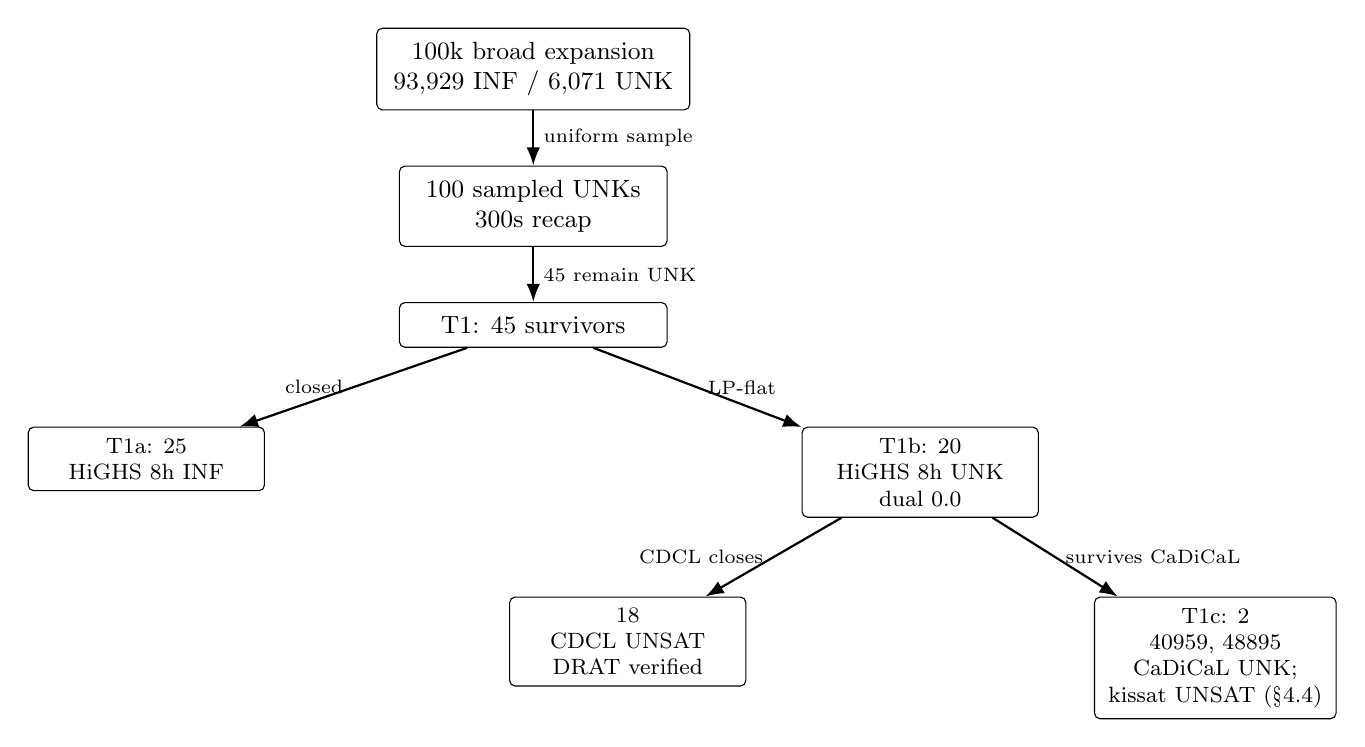
\begin{tikzpicture}[
  >=Latex,
  node distance=7mm and 8mm,
  box/.style={
    draw,
    rounded corners=2pt,
    align=center,
    inner xsep=6pt,
    inner ysep=5pt,
    font=\small,
    minimum width=34mm
  },
  smallbox/.style={
    draw,
    rounded corners=2pt,
    align=center,
    inner xsep=5pt,
    inner ysep=4pt,
    font=\footnotesize,
    minimum width=30mm
  },
  edge/.style={->, thick}
]
\node[box] (broad) {100k broad expansion\\93,929 INF / 6,071 UNK};
\node[box, below=of broad] (recap) {100 sampled UNKs\\300s recap};
\node[box, below=of recap] (t1) {T1: 45 survivors};
\node[smallbox, below left=10mm and 17mm of t1] (t1a) {T1a: 25\\HiGHS 8h INF};
\node[smallbox, below right=10mm and 17mm of t1] (t1b) {T1b: 20\\HiGHS 8h UNK\\dual 0.0};
\node[smallbox, below left=10mm and 7mm of t1b] (cdcl) {18\\CDCL UNSAT\\DRAT verified};
\node[smallbox, below right=10mm and 7mm of t1b] (t1c) {T1c: 2\\40959, 48895\\CaDiCaL UNK;\\kissat UNSAT (\S4.4)};

\draw[edge] (broad) -- node[right, font=\scriptsize] {uniform sample} (recap);
\draw[edge] (recap) -- node[right, font=\scriptsize] {45 remain UNK} (t1);
\draw[edge] (t1) -- node[left, font=\scriptsize] {closed} (t1a);
\draw[edge] (t1) -- node[right, font=\scriptsize] {LP-flat} (t1b);
\draw[edge] (t1b) -- node[left, font=\scriptsize] {CDCL closes} (cdcl);
\draw[edge] (t1b) -- node[right, font=\scriptsize] {survives CaDiCaL} (t1c);
\end{tikzpicture}

}
\caption{Funnel from the retained 100k broad expansion batch to the final
two-chunk T1c residual. T1 is a 45-chunk subset produced by recapping a
uniform random 100-chunk sample of the 6,071 broad UNKNOWN chunks at
300 seconds (sampling seed 5230). T1c, which survives CaDiCaL, is later refuted by kissat
4.0.4 (§4.4).}
\label{fig:t1-funnel}
\end{figure}

\subsection{The window-cardinality A/B}\label{the-window-cardinality-ab}

The single most impactful intervention in the campaign was adding
window-cardinality inequalities derived from the OEIS A003002 b-file.
For every window $[a,a+L-1]\subseteq[1,212]$ and every length $L$ with
$r_3(L)<\min(L,K)$, we add $\sum_{i=a}^{a+L-1}x_i\leq r_3(L)$. For
$N = 212$, $K = 44$ this generates 22,154 inequalities, on top of the
11,130 3-AP triple inequalities and the symmetry-breaking lex
constraint.

We measured the effect on three batches of varying size:

{\def\LTcaptype{none} % do not increment counter
\begin{longtable}[]{@{}lr
  >{\raggedleft\arraybackslash}p{(\linewidth - 10\tabcolsep) * \real{0.1600}}
  >{\raggedleft\arraybackslash}p{(\linewidth - 10\tabcolsep) * \real{0.1600}}
  r@{}}
\toprule\noalign{}
Batch & Chunks & UNK without window-bounds & UNK with window-bounds & Reduction \\
\midrule\noalign{}
\endhead
\bottomrule\noalign{}
\endlastfoot
$[575, 675)$ & 100 & 27.00\% & 0.00\% & $-27.0$ pp \\
$[1575, 11575)$ & 10,000 & 30.33\% & 1.65\% & $-28.7$ pp \\
$[11575, 111575)$ & 100,000 & n/a & 6.07\% & --- \\
\end{longtable}
}

Both controlled A/Bs show a roughly 28-percentage-point reduction in
\texttt{UNKNOWN} rate at the 60-s broad wall cap. Although the window
inequalities are logically implied by the complete 3-AP model, they produce
a materially stronger formulation for propagation at this problem size. In
the retained logs they also lowered total broad-pass solver time, because many
formerly hard chunks closed early under the extra bounds.

The $[575, 675)$ A/B is a 100-chunk subrange of the calibration range
reported in §3.1; the difference between its 27.00\% no-window \texttt{UNK} rate
and the calibration range's 20.10\% reflects the structural non-uniformity of
chunk-ID space rather than a change in model configuration.

However, the \texttt{UNK} rate is non-monotone in the chunk-ID range: the small
controlled A/B on $[575, 675)$ closes to 0\%, the 10k bounded batch
sits at 1.65\%, and the 100k expansion batch sits at 6.07\%. This
indicates that the chunk-ID space is structurally non-uniform --- later
chunk IDs (which encode different witness-pin assignments) are harder
in a way that window-bounds do not fully compensate for. The bucket
analysis in §4.1 quantifies this non-uniformity.

\subsection{Solver configuration and engineering}\label{solver-configuration-and-engineering}

All CP-SAT calls use the following configuration unless explicitly
overridden in an experiment:

\begin{itemize}
\tightlist
\item
  Model: decision-mode $\sum_i x_i = 44$, 11,130 3-AP linear
  inequalities, 22,154 window-cardinality inequalities, lex
  reflection symmetry break, endpoint forcing $x_1=x_{212}=1$.
\item
  Branch strategy: variable selection by AP-incidence degree, minimum-value
  selection, and fixed-search mode to disable CP-SAT's portfolio.
\item
  Solver: OR-Tools CP-SAT \cite{or-tools}, 8 workers per task, fixed solver seed
  and fixed search parameters, wall cap as noted (most commonly 60-s
  for broad, 300-s and 600-s for recap experiments).
\end{itemize}

The retained Unity environment used Python 3.12, OR-Tools 9.15.6755,
HiGHS 1.14.0, and PySAT 1.9.dev4. The no-proof \texttt{pysat:auto}
path selected the \texttt{cadical195} backend; the later native solver was
kissat 4.0.4. Exact command lines and environment captures accompany the
released logs.

The SLURM emitter, shard collector, tail emitter, and proof-state manager
implement the workload pipeline. Output is
written as line-delimited JSON with one record per chunk; shards are
written to a temporary path and atomically renamed on completion so
that partial output from killed tasks cannot corrupt downstream
collection. The full campaign is reproducible end-to-end via the
\texttt{unity\_handoff.sh} driver.

\subsection{Zero FEASIBLE across the campaign}\label{zero-feasible-across-the-campaign}

Aggregating across the monolithic baseline (§3.1), the broad pass, the
refinement loop, the recap studies, the lever experiments of §3.6, the
HiGHS attack of §4.3, the CDCL/SAT and proof-producing reruns of §4.3,
and the kissat re-attack and T2 survey of §4.4, the campaign solved
millions of \texttt{(N,\ K,\ fixed\_in,\ fixed\_out)} subproblems,
including prefix-closure work not tabulated above. The number of
subproblems returning \texttt{FEASIBLE} or \texttt{SAT} is \textbf{zero}.

The \texttt{FEASIBLE} count is the only signal that would directly disprove
$r_3(212) \leq 43$; its absence does not constitute a proof of the upper
bound, but it is strong empirical support, especially given that the
campaign forced the endpoints 1 and 212, which any 44-set must contain by
the known value $r_3(211) = 43$, and then explored a depth-24 prefix of the
verified 43-witness in the processed chunk ranges. Within the processed
expansion range, a 44-element 3-AP-free subset of $[1, 212]$, if one existed,
would have to lie in the 6,071 unresolved broad \texttt{UNKNOWN} chunks (or in
their deeper refinements). Globally, the much larger unprocessed remainder of
the full depth-24 sweep remains open as well.

\subsection{Search-tuning levers and their effect sizes}\label{search-tuning-levers-and-their-effect-sizes}

We tested five CP-SAT-side search-tuning levers. The
full lever inventory, including the HiGHS substitution and the
pair-AND Tseitin experiment, is consolidated in §4.5; here we report
only the three CP-SAT-side levers that operate at the broad layer.

{\def\LTcaptype{none} % do not increment counter
\begin{longtable}[]{@{}
  >{\raggedright\arraybackslash}p{(\linewidth - 10\tabcolsep) * \real{0.1800}}
  >{\raggedright\arraybackslash}p{(\linewidth - 10\tabcolsep) * \real{0.2800}}
  >{\raggedright\arraybackslash}p{(\linewidth - 10\tabcolsep) * \real{0.1800}}
  rr@{}}
\toprule\noalign{}
Lever & Mechanism & Bucket & Baseline UNK & Treatment UNK \\
\midrule\noalign{}
\endhead
\bottomrule\noalign{}
\endlastfoot
Split-vars reorder & Permute the depth-24 prefix so hot pins (values \texttt{\{68,\ 75,\ 70,\ 76,\ 91\}}) lead & $[61575, 66575)$ & 13.60\% & 12.96\% \\
Wall-cap extension 60 s to 300 s & Same model, same prefix, longer per-chunk budget & random 100 from expansion \texttt{UNKNOWN} & 100.00\% & 45.00\% \\
Recursive deepening & Refine \texttt{UNK} to depth 64 at 600-s cap & 6 L3 residuals & 100.00\% & 0.00\% \\
\end{longtable}
}

The reorder lever was tested for completeness but is expected to be a
null result on principle: the depth-24 broad split iterates over the
\texttt{2\^{}24} IN/OUT prefix assignments, and within-prefix variable ordering
does not change the set of surviving chunks under AP-prefix pruning
--- only the order in which they are emitted to SLURM. The within-noise
result confirms this.

The wall-cap extension lever moves the residual substantially on the
first doubling but exhibits a saturating closure curve under further
extension. The 60 s, 120 s, and 300 s series is analyzed in §4.2; in
brief, the marginal close-rate per additional second of wall drops
sharply past 300-s, which is why the campaign did not pursue
600-s or 1200-s broad-layer reruns on the full 6,071-chunk
expansion residual.

The recursive-deepening lever, applied locally to small residual sets,
reliably closes individual deep \texttt{UNK} chunks (6/6 at the L4 level
in §3.1). But the levers it implies --- picking the next-degree split
variables and re-solving up to \texttt{2\^{}8} descendant assignments at a longer wall ---
do not
generalize cheaply to the full 6,071-chunk expansion residual. A
naïve depth-32 rerun on every expansion \texttt{UNK} would emit roughly
1.5 million subproblems and require an order of magnitude more CPU
time than the original broad pass, with no guarantee of closing the
hard core analyzed in §4.

\subsection{Compute budget}\label{compute-budget}

The dominant retained costs are the 100k broad expansion, the
sample-500 refinement, and the full-T1 long-wall HiGHS audit; the CDCL and
certificate diagnostics are comparatively cheap. The total retained-log
estimate is roughly 8,710 worker-hours; Appendix~\ref{app:compute}
itemizes the accounting per campaign layer. A full depth-24 sweep of
the 12,582,912 AP-pruned chunks of the witness-split lattice was outside
this campaign's budget under the CP-SAT-first parameters used here; §5.3
reprices the sweep in light of the kissat results of §4.4, which shift
the bottleneck from search to proof logging and verification at scale.

\section{The structural hard pocket}\label{the-structural-hard-pocket}

The headline empirical finding of the campaign is not the absence of a 44-element
3-AP-free subset of $[1, 212]$ --- which we expected from the OEIS A003002
extrapolation $r_3(212) = 43$ --- but the existence, stratification, and
eventual collapse of a small, robust subset of broad subproblems that
resisted every solver we initially threw at them. We refer to this subset
as the \emph{hard pocket}. This section characterizes it empirically,
summarizes the interventions in the order we tried them, and ends with the
kissat re-attack that resolved it (§4.4) --- a resolution that refutes our
own working hypothesis (§4.6) and shows that the observed boundary depends
on solver implementation and configuration.

\subsection{Empirical signature on the broad population}\label{empirical-signature-on-the-broad-population}

The 100,000-chunk window-bound broad batch over chunk-id range
$[11575, 111575)$ produced 93,929 \texttt{INFEASIBLE} chunks, 6,071 \texttt{UNKNOWN}
chunks, and 0 \texttt{FEASIBLE} chunks under a 60-second per-chunk wall cap. The
6.07\% UNKNOWN rate is non-uniform in two distinct senses.

\textbf{Bucket non-uniformity.} Partitioned into twenty 5,000-chunk buckets, the
UNKNOWN rate varies from 1.64\% to 13.60\%, with the worst bucket
$[61575, 66575)$ at 13.60\%. The longest contiguous UNKNOWN run found in this
batch was length 27 at chunk IDs 98277..98303; many other runs have length
around 15. These contiguous runs are consistent with joint structural
properties of the depth-24 witness-pin assignment affecting closure time;
they do not by themselves separate structural effects from runtime variation.

\textbf{Pin-OUT enrichment.} For each of the 24 broad-split witness variables we
computed the conditional UNKNOWN rate given that variable's IN/OUT assignment
in the chunk. Five variables --- values 68, 75, 70, 76, 91, all in the
dense middle cluster $[67, 91]$ of the verified 43-witness --- show a strong
asymmetry: their pooled conditional UNKNOWN rate is roughly 2.4\% when pinned IN
and 9.7\% when pinned OUT, an odds ratio of approximately 4.4. The signal is consistent
across the five values. We refer to a chunk in which all five hot pins are
forced OUT as a \emph{middle-out chunk}. Middle-out chunks account for a
disproportionate share of the UNKNOWN tail of the broad batch.

\subsection{The 300s-resistant tail does not collapse}\label{the-300s-resistant-tail-does-not-collapse}

To test whether the broad-pass UNKNOWNs were merely ``slow'' rather than
structurally hard, we ran two wall-cap recalibration experiments on a uniform
random sample of 100 UNKNOWN chunks drawn from the 6,071 baseline (seed
5230). The
results show a saturating, not exponential, closure curve:

{\def\LTcaptype{none} % do not increment counter
\begin{longtable}[]{@{}rrrr@{}}
\toprule\noalign{}
Wall cap & INFEASIBLE & UNKNOWN & Close rate over baseline \\
\midrule\noalign{}
\endhead
\bottomrule\noalign{}
\endlastfoot
60 s & 0 & 100 & 0\% \\
120 s & 31 & 69 & 31\% \\
300 s & 55 & 45 & 55\% \\
\end{longtable}
}

Going from 60 s to 120 s closed 31 chunks. Increasing the cap further to
300 s closed 24 more. The marginal gain per additional second decreased on
this sample, and 45 chunks remained unresolved; these three points do not
support a reliable extrapolation beyond 300 s.

We applied the same structural mining procedure (single-pin, pair, and triple
log-odds enrichment relative to a matched \texttt{INFEASIBLE} sample) to the 45
\texttt{UNKNOWN} chunks that survived the 300s cap. The broad pin-OUT signature
weakens substantially. The best high-coverage pair, $[91=OUT, 48=OUT]$, covers
66.67\% of the survivors, but its enrichment over matched
\texttt{INFEASIBLE} controls is modest. Top triples are more selective but
each covers only a handful of cases. Hamming-distance
clustering of survivor \texttt{fixed\_in} sets shows multiple small clusters rather
than a single dominant niche. We interpret this as evidence that the
300s-resistant subproblems share moderate pin-OUT structure but spread
across many distinct sub-pockets of the depth-24 assignment lattice.

\subsection{HiGHS resistance and the CDCL break}\label{highs-resistance-and-the-cdcl-break}

The 300s-resistant pocket might in principle be specific to the tested
CP-SAT formulation and search policy. To test a substantially different
solver architecture, we re-attacked all 45 survivors with
the HiGHS open-source MIP solver \cite{huangfu-hall-2018-highs}, which combines branch-and-bound, LP
relaxation, presolve, cutting planes, and primal heuristics. We used a
one-hour wall cap per chunk, 8 threads per chunk, and the identical
constraint set
(decision-form $\sum x_i = 44$, all 11,130 3-AP triple inequalities, all
22,154 window-cardinality inequalities, plus the broad chunk's \texttt{fixed\_in}
and \texttt{fixed\_out} assignments tightened into variable bounds).

The one-hour result was negative:

The two rows in the following table are not a common-sample comparison: the
HiGHS attack targets precisely the 45 chunks that survived the 300-s
CP-SAT recap, i.e.~the harder subset of the 100 recap inputs.

{\def\LTcaptype{none} % do not increment counter
\begin{longtable}[]{@{}
  >{\raggedright\arraybackslash}p{(\linewidth - 12\tabcolsep) * \real{0.1600}}
  >{\raggedright\arraybackslash}p{(\linewidth - 12\tabcolsep) * \real{0.2200}}
  rrr
  >{\raggedright\arraybackslash}p{(\linewidth - 12\tabcolsep) * \real{0.2200}}@{}}
\toprule\noalign{}
Solver & Constraints & Wall cap & Closed (INF) & UNKNOWN & Aggregate solver wall time \\
\midrule\noalign{}
\endhead
\bottomrule\noalign{}
\endlastfoot
CP-SAT, window-bounds & 3-AP + window + symmetry & 300 s & 55 / 100 & 45 / 100 & bounded by \textasciitilde8.3 wall-h \\
HiGHS, window-bounds & 3-AP + window + endpoint & 3,600 s & \textbf{0 / 45} & 45 / 45 & 45.0 wall-h \\
\end{longtable}
}

Across 162,003 solver-seconds and 3,181,316 explored MIP nodes, HiGHS did
not close a single chunk. No \texttt{FEASIBLE} row appeared. Because the model
was posed as a zero-objective feasibility problem with $\sum_i x_i=44$, the
recorded objective and dual bounds of $0.0$ are non-diagnostic; this experiment
measures MIP closure under the tested formulation, not the quality of a
maximization-model LP bound.

We then re-attacked all 45 T1 chunks under an extended 8-hour HiGHS wall,
with progress logging enabled. The result is mixed: 25/45 chunks closed
\texttt{INFEASIBLE}, while 20/45 returned \texttt{UNKNOWN} at the full cap. We call
this 20-chunk HiGHS-resistant subset \textbf{T1b}. The audit consumed
901,073 solver-seconds and 25,196,448
MIP nodes.

To test whether T1b is invariant under solver architecture more broadly, we
re-attacked it with a CDCL/SAT solver (CaDiCaL via PySAT
\cite{biere-cadical,pysat-2018}, single-threaded,
4-hour wall, encoding restricted to 3-AP triples + cardinality + chunk pins;
no window-cardinality clauses). CDCL closed 18/20 chunks \texttt{UNSAT}. We call
the surviving 2-chunk residual \textbf{T1c} = $\{40959, 48895\}$. A T1c diagnostic
at extended wall (12 h pure CDCL) and with totalizer-encoded window
constraints for lengths \texttt{\{31,\ 100,\ 199\}} (4 h) also returned \texttt{UNKNOWN} on
both chunks. At that point in the campaign, T1c appeared resistant to
every tested configuration; §4.4 reports the re-attack that overturned this.

A proof-producing rerun of the 18 CDCL-UNSAT chunks initially emitted DRAT
proofs for 17 chunks; the remaining chunk, 32735, required a larger-memory
proof rerun and then also emitted a DRAT proof. Independent \texttt{drat-trim}
verification confirmed all 18/18 emitted proofs. The final two certificates
were the slowest: 63231 verified in 49,758.11 seconds and 32735 verified
in 80,960.68 seconds under the final 24-hour verifier pass
\cite{heule-hunt-biere-drat-2014,cruz-filipe-lrat-2017}.

The picture after the CaDiCaL pass is configuration-specific but sharp:
the tested CP-SAT and HiGHS formulations leave all of T1b unresolved, while
the tested CaDiCaL configuration closes 18/20 of those chunks, all with
independently verified proofs. The residual was T1c, of size 2.

\subsection{Kissat closes T1c: a solver-configuration separation}
\label{kissat-closes-t1c}

The CaDiCaL result left open whether T1c marks the edge of the tested CDCL
configuration or only of one implementation. We therefore re-attacked both
chunks with kissat 4.0.4 \cite{biere-cadical}, single-threaded, on the same
pure 3-AP/cardinality encoding (no window clauses), with DRAT logging
enabled. Both chunks were refuted, and both refutations are certified
end-to-end: against sha256-pinned formula files, chunk 40959 solves in
23,191 s with independent \texttt{drat-trim} verification in 41,127 s,
and chunk 48895 solves in 10,083 s with verification in 16,153 s. (An
initial kissat run on the same encoding had already refuted both, in
14,204.9 s and 17,621.7 s, emitting proofs of 17.4 and 14.3 GB; the
certified rerun re-solved and re-verified against the same pinned
formula file per chunk to establish clean certificate provenance.)
Every solve sits well inside the 12-hour budget under which the CaDiCaL
attempts failed. One caveat on attributing this gap: the CaDiCaL
attacks ran through PySAT's bundled build with default configuration,
so part of the separation may reflect build vintage or configuration
defaults rather than core search differences; the released instances
make it straightforward to re-measure against any solver build. (A
windowed kissat variant exceeded the 16 GB encode-time memory budget on
both chunks and produced no solver result.)

To measure whether the kissat/CaDiCaL gap is specific to T1c or generic
across the broad residual, we ran a kissat survey on a fresh uniform
random 100-chunk sample of the 6,071 T2 \texttt{UNKNOWN}s (seed 42; 2-hour cap,
no proof logging): 99/100 closed \texttt{UNSAT}, with median solve time
121.7 s and maximum 2,408.8 s; the single survivor (chunk 98301) hit
the cap. The whole survey consumed 34,819.8 solver-seconds --- less
than ten CPU-hours for 99 closures of subproblems that all survived the
campaign's 60-second CP-SAT broad pass with window bounds. The binomial
Wilson 95\% interval for the within-cap closure probability is approximately
94.6\%--99.8\%; this interval describes the sampled T2 population and does
not establish behavior on T3. Together with the
T1c closures, this collapses the hard pocket as a solver-independent
phenomenon. What remains true, and is now cleanly isolated: (i) the tested
CP-SAT and HiGHS configurations leave the same T1b set unresolved; (ii)
within CDCL, implementation and configuration matter at the hard end ---
the two chunks that defeat the tested CaDiCaL setup at 12 h fall to kissat
in the initial run within 5 h and in the certificate-pinned rerun within
6.5 h; and (iii) the tiers T1a/T1b/T1c retain their value as a graded,
ground-truth-verifiable ladder that separates solver technologies at
three distinct heights.

\subsection{Levers tested and their outcomes}\label{levers-tested-and-their-outcomes}

For completeness, we record every search-tuning lever we tested on the hard
bucket $[61575, 66575)$ or the 300s-resistant subset. The CP-SAT/MIP-side
tuning levers did not remove the hard pocket; the one qualitative exception is
the CNF/CDCL switch, which closes most of T1b and therefore narrows, rather
than merely tunes, the residual.

{\def\LTcaptype{none} % do not increment counter
\begin{longtable}[]{@{}
  >{\raggedright\arraybackslash}p{(\linewidth - 6\tabcolsep) * \real{0.2600}}
  >{\raggedright\arraybackslash}p{(\linewidth - 6\tabcolsep) * \real{0.3200}}
  >{\raggedright\arraybackslash}p{(\linewidth - 6\tabcolsep) * \real{0.4200}}@{}}
\toprule\noalign{}
Lever & Mechanism & Result \\
\midrule\noalign{}
\endhead
\bottomrule\noalign{}
\endlastfoot
Window-cardinality (OEIS A003002) & Add $\sum x \leq r_3(L)$ for each window & UNKNOWN rate on full 10k batch: 30.33\% to 1.65\%. Strong but plateaus. \\
Split-vars reorder (hot pins first) & Permute the depth-24 split prefix & 13.60\% to 12.96\% on the worst bucket. Within the observed noise. \\
Wall-cap extension & 60 s to 300 s on the broad pass & Diminishing closure gains, see §4.2. \\
Targeted pair-AND Tseitin propagators & Explicit \texttt{pair{[}a,c{]}\ =\ x{[}a{]}∧x{[}c{]}} BoolVars on midpoints in $[67, 91]$ & Control 67.84s, treatment 71.75s on a sampled residual. No effect. \\
Recursive deepening & Refinement at depths 40, 48, 56 & All 500 stratified-sample base chunks close, but with a non-trivial tail; the final six level-3 residuals needed up to 599.74s at the 600s cap. \\
HiGHS MIP with LP/cut machinery & Replace CP-SAT entirely & 0/45 closed at 1 hour; 25/45 closed in the full 8-hour audit, while 20/45 remained unresolved. \\
Pure CDCL/SAT & Encode T1b as CNF with 3-AP clauses + cardinality + pins, no windows & 18/20 HiGHS-resistant chunks closed \texttt{UNSAT} in 4 hours; 2/20 remained \texttt{UNKNOWN}; no \texttt{SAT} rows. \\
Kissat re-attack (§4.4) & Same mathematical CNF encoding, kissat 4.0.4 & Both T1c chunks refuted and independently verified; 99/100 of a fresh T2 sample closed within 2 h. \\
\end{longtable}
}

The pair-AND result is worth a closer note. The added constraints are
mathematically redundant with the existing 3-AP triple inequalities --- they
encode the same forbidden configurations, just with an explicit Tseitin
variable per pair. The hope was that this would give CP-SAT more
``propagation hooks'' in the structural pocket. The negative result is
consistent with the broader picture: the pocket's hardness is not an
encoding issue, it is a search-space issue.

\subsection{A refuted working hypothesis about the pocket}\label{a-refuted-hypothesis-about-the-pocket}

During the campaign we maintained the working hypothesis that T1c marked a
solver-independent hard core under practical wall caps. That hypothesis was
based on repeated non-closure by CP-SAT, HiGHS, and the tested CaDiCaL setup;
it was not a theorem about proof complexity or the LP relaxation. Kissat
4.0.4 refuted the hypothesis by finding multi-gigabyte DRAT proofs for both
chunks, which \texttt{drat-trim} independently verified.

The corrected picture is narrower and more reproducible: T1c separates the
specific CaDiCaL and kissat configurations tested here. Because the CaDiCaL
runs used PySAT's bundled build and defaults, the experiment does not isolate
which implementation or configuration choice explains the separation. A
controlled comparison on the archived, byte-identical CNFs is therefore a
natural follow-up. Likewise, a meaningful claim about LP-relaxation strength
requires a maximization model with a nonzero objective; the zero-objective
HiGHS feasibility runs reported here cannot provide that evidence.

\subsection{\texorpdfstring{What this means for $r_3(212)$}{What this means for r\_3(212)}}\label{what-this-means-for-r_3212}

The combined CP-SAT, HiGHS, CaDiCaL, and kissat evidence --- 0
\texttt{FEASIBLE}/\texttt{SAT} rows across millions of subproblems, every
audited hard-pocket chunk closed \texttt{UNSAT}, and 99/100 of a fresh
broad-residual sample closed within 2 hours --- strongly supports the
OEIS-conjectured value $r_3(212) = 43$, and the kissat results
substantially change the outlook on proving it. The lower bound
$r_3(212) \geq 43$ from the verified witness in §2 is unaffected; the trivial
upper bound $r_3(212) \leq 44$ follows from monotonicity and OEIS
$r_3(211) = 43$, so the gap between our certified bounds is exactly one.

What blocks the upper bound is complete coverage and certification of the
remaining search space: closing it requires certifying the full
12,582,912-chunk depth-24 sweep (T3), of which this campaign processed the
100,000-chunk expansion plus samples. The T2 pilot's observed rate
(99/100 within 2 h/chunk, single-core) suggests that a larger kissat sweep
is plausible, but one sampled T2 survivor and the unprocessed T3 remainder
leave the cost and tail behavior uncertain. A certified sweep would be
of the same general character as the Pythagorean-triples and Schur-five
campaigns \cite{heule-kullmann-marek-2016,heule-2018-schur}, with the
witness-split generator providing the cube decomposition. We release the
benchmark instances and generator in §5 so that this sweep, or a sharper
per-chunk method, can be attempted directly.

\section{Open problem and benchmark release}\label{open-problem-and-benchmark-release}

The campaign establishes strong empirical support for $r_3(212) = 43$
(§3.5, §4.4). Kissat closes every audited hard instance and 99\% of a
fresh residual sample, while complete coverage and certification of T3
remain open (§4.4). This
section states the residual problem cleanly and releases the instances
as a tiered benchmark --- both as a concrete path toward R3-212-UB and as
a solver-grading ladder for the tested CP-SAT, HiGHS, and CDCL
configurations.

\subsection{Statement of the open problem}\label{statement-of-the-open-problem}

\begin{quote}
\textbf{Problem (R3-212-UB).} Let $A\subseteq[1,212]$ with $|A|=44$. Determine
whether there exists $A$ containing no nontrivial 3-term arithmetic
progression. The verified 43-element witness in
\texttt{results/N212\_K43\_witness.json} (§2.1) and the value $r_3(211) = 43$
from OEIS A003002 jointly imply that any such $A$ must contain both
endpoints 1 and 212. Equivalently, either exhibit one such $A$
or certify the infeasibility of the decision problem
$\sum_i x_i = 44$ over the 3-AP constraint family on $[1, 212]$
with $x_1=x_{212}=1$.
\end{quote}

A solution to R3-212-UB resolves the unit gap $r_3(212)\in\{43,44\}$
in either direction. Our multi-million-subproblem CP-SAT campaign, the
45-instance HiGHS attack, and the CaDiCaL/kissat re-attacks returned 0
\texttt{FEASIBLE}/\texttt{SAT} rows, which is evidence for the
infeasibility branch but not a proof. The benchmark instances released
below pinpoint the subproblems on which solver technologies diverge.

\subsection{Benchmark instance tiers}\label{benchmark-instance-tiers}

We release five benchmark tiers. Each JSONL row records the chunk ID,
fixed assignments, witness-pin prefix, solver status, and timing data; the
common constraint family (3-AP triples, endpoint forcing, and OEIS window
bounds) is reconstructed by the repository scripts. The tiers form a ladder
from the smallest solver-resistant pocket to the full upper-bound proof.

{\def\LTcaptype{none} % do not increment counter
\begin{longtable}[]{@{}
  >{\raggedright\arraybackslash}p{(\linewidth - 10\tabcolsep) * \real{0.1000}}
  >{\raggedright\arraybackslash}p{(\linewidth - 10\tabcolsep) * \real{0.2000}}
  r
  >{\raggedright\arraybackslash}p{(\linewidth - 10\tabcolsep) * \real{0.2400}}
  >{\raggedright\arraybackslash}p{(\linewidth - 10\tabcolsep) * \real{0.2400}}@{}}
\toprule\noalign{}
Tier & Artifact & Size & Resistance level & Recommended target \\
\midrule\noalign{}
\endhead
\bottomrule\noalign{}
\endlastfoot
T1a & T1a JSONL & 25 chunks & closed by HiGHS at 8h & reference / regression test \\
$\mathrm{T1b}\setminus\mathrm{T1c}$ & T1b-minus-T1c JSONL & 18 chunks & HiGHS-resistant; closed by CDCL; all 18/18 emitted DRAT proofs verified by \texttt{drat-trim} & certified CDCL benchmark \\
T1c & T1c JSONL & 2 chunks & resist CP-SAT, HiGHS LP-MIP, CaDiCaL @ 12h; refuted by kissat 4.0.4, DRAT-certified & CDCL-implementation calibration point \\
T2 & T2 JSONL & 6,071 chunks & survived 60-s CP-SAT broad pass with window bounds & full closure of the expansion residual \\
T3 & deterministic generator & 12,582,912 chunks & unprocessed remainder of the witness-split lattice & full upper-bound proof \\
\end{longtable}
}

The concrete filenames are \path{results/N212_K44_t1a25.jsonl},
\path{results/N212_K44_t1b_minus_t1c.jsonl},
\path{results/N212_K44_t1c2.jsonl}, and
\path{results/N212_K44_window100k_unknowns.jsonl}.

Tier T1c is the benchmark's calibration point for CDCL implementations:
the two chunks defeat CaDiCaL at a 12-hour wall and fall to kissat 4.0.4
well within that budget, with end-to-end certified DRAT proofs (§4.4).
The pair is useful as a compact regression and configuration-calibration
set; lower solve or verification cost than the reported runs is a directly
comparable benchmark improvement.

Tier T2 is the canonical ``close the campaign at the broad layer''
target: closing all 6,071 chunks of the 100k expansion batch is
necessary, though not sufficient, for a full upper-bound proof. The
kissat pilot (99/100 within 2 h/chunk at median 121.7 s, §4.4)
extrapolates to roughly 500 single-core CPU-hours of solving for the
full tier, plus proof-logging and verification overhead and whatever
the $\approx 1\%$ tail beyond the 2-hour horizon costs; chunk 98301 ---
the one pilot survivor --- is the natural first target for anyone
probing that tail.

Tier T3 is the full upper-bound certificate: closing the entire
depth-24 AP-pruned sweep. The instance generator (§2.2) emits the
required chunks deterministically from the witness file and the
OEIS b-file; the storage cost of the full sweep is dominated by
output rather than input.

\subsection{Minimum-viable proof requirements}\label{minimum-viable-proof-requirements}

A formal proof of $r_3(212)\leq 43$ from the released benchmark requires:

\begin{enumerate}
\def\labelenumi{\arabic{enumi}.}
\tightlist
\item
  \textbf{Closure of tier T3.} Every chunk in the depth-24 AP-pruned
  sweep must return \texttt{INFEASIBLE} under a verified solver, or one
  chunk must return a \texttt{FEASIBLE} 44-element witness.
\item
  \textbf{Solver verification.} Every infeasibility result used in the proof
  must be justified by a machine-checkable certificate (DRAT, LRAT, or an
  equivalent proof format) checked by a trusted or formally verified checker.
  Agreement between two unverified solvers is useful validation but is not a
  formal certificate. Section 6.2 records the present gaps.
\item
  \textbf{Constraint-set verification.} The 11,130 3-AP triple
  inequalities, the 22,154 window-cardinality inequalities, and
  the endpoint forcing must be checked against the formal
  definition of $r_3(N)$. The verifier \texttt{r3\_verify.py} performs
  this check on any candidate witness; an analogous check for the
  constraint generation is included in the repository.
\end{enumerate}

The minimum-viable result short of a full proof is the certified
closure of tier T2: verified proofs for all 6,071 broad-residual
chunks. The kissat pilot (§4.4) prices the solving at roughly 500
single-core CPU-hours (extrapolating the pilot's mean closed-chunk
time to all 6,071 chunks), with proof emission, verification, and the
$\approx 1\%$ hard tail as the real cost drivers. This estimate is a
planning figure from one sample, not a bound on the cost of T2 or T3. A
separate optimization-form MIP experiment that maximizes $\sum_i x_i$
would be needed to measure meaningful primal and dual bounds on T1b.

\subsection{Approaches we could not test}\label{approaches-we-could-not-test}

The following techniques are plausibly stronger than CP-SAT and HiGHS
on this pocket but were outside the scope of our campaign. We flag
them as natural follow-on directions:

\begin{itemize}
\tightlist
\item
  \textbf{Fourier-analytic upper bounds.} Behrend-style constructions
  achieve $r_3(N) = N · exp(-c·sqrt(log N))$ lower bounds; a
  matching Fourier-analytic upper bound for small $N$ would give a
  certificate independent of combinatorial search. The Bloom--Sisask
  framework for $r_3(N) = O(N / (log N)^\{1+c\})$ is asymptotic but
  the underlying density-increment machinery may yield finite-$N$
  bounds tighter than the OEIS window-cardinality family.
\item
  \textbf{Multi-window partition bounds.} OEIS A003002 is used here as
  a single-window family $\sum_{i=a}^{a+L-1}x_i\leq r_3(L)$. A
  partition-cardinality bound across multiple disjoint windows of
  varying length might cut the LP relaxation more aggressively
  than any single-window family.
\item
  \textbf{SAT with proof logging at scale.} A pure CNF encoding closed
  18/20 T1b chunks under CaDiCaL (all DRAT-verified) and, per §4.4, the
  remaining two under kissat 4.0.4 (also DRAT-verified). The
  research target has therefore moved from single instances to the
  certified sweep: proof-producing kissat over all of T2 and ultimately
  T3, with verification and archival at Pythagorean-triples scale
  \cite{heule-kullmann-marek-2016}. Open per-instance questions remain
  at the margins --- e.g.\ chunk 98301, the one pilot survivor, and
  whether alternative cardinality encodings shrink the multi-GB
  certificates of the hardest chunks.
\item
  \textbf{Lean/formal-proof-search benchmark.} The repository now includes a compact
  Lean 4 / Mathlib 4 formalization \cite{lean4-2021,mathlib4} under \texttt{lean/}: shared definitions
  (\texttt{R3Base.lean}), the verified 43-witness statement
  (\texttt{R3\_212\_Witness.lean}), and two AlphaProof-style T1c targets
  (\texttt{R3\_T1c\_40959.lean}, \texttt{R3\_T1c\_48895.lean}) with the expected answer \texttt{false}.
  These files are intended as a starting point for an A003002 / $r_3(N)$ entry
  in formal-conjecture repositories \cite{formal-conjectures}. Recent AlphaProof Nexus-style workflows
  have resolved Erdős problems of comparable complexity at low per-problem cost
  when a Lean target exists \cite{tsoukalas-alphaproof-nexus-2026}, so T1c is well-shaped for that workflow.
\item
  \textbf{Custom branch-and-bound.} A solver that exploits problem-
  specific symmetries and dominance relations --- for instance,
  reflection symmetry after endpoint forcing, or domination of one
  window-bound by another at specific fixed-pin configurations ---
  could prune branches that neither CP-SAT nor HiGHS recognize as
  redundant.
\item
  \textbf{Symmetric Difference Encoding / Lasserre hierarchy at low
  degree.} A degree-4 or degree-6 SDP relaxation of the
  3-AP-free constraint might separate the surviving T1 instances
  from feasibility where the LP relaxation cannot.
\end{itemize}

We do not advocate for any single direction. The benchmark release
is intended to let specialists pick the technique closest to their
toolkit.

\subsection{Reproducibility and release}\label{reproducibility-and-release}

The campaign code, configuration, and result logs are released at
the repository accompanying this preprint. Specifically:

\begin{itemize}
\tightlist
\item
  All Python sources implementing the architecture of §2 are present
  with module-level documentation.
\item
  The SLURM scripts (\texttt{submit\_*.sbatch}) and the driver
  \texttt{unity\_handoff.sh} reproduce the full campaign on any
  SLURM-compatible cluster with OR-Tools and \texttt{highspy} installed.
\item
  The verified 43-witness, the OEIS A003002 b-file used for window
  bounds, the broad-pass result logs, the recap residuals, the
  HiGHS attack logs, the T1a/T1b/T1c benchmark JSONLs, the Lean T1c
  proof-search targets, environment/version captures for the main solver stack,
  and the scripts needed to generate T3 are included in the repository or
  its associated artifact archive.
\item
  Existing single-instance entry points (\texttt{r3\_split\_cpsat.py} and
  \texttt{r3\_highs\_attack.py}, and \texttt{r3\_sat\_attack.py}) can rerun any row of T1c,
  T1b, or T2 by chunk ID.
\end{itemize}

The large solver artifacts are archived on Zenodo at
\url{https://doi.org/10.5281/zenodo.20463334}. Version 1 contains the
CNF/DRAT proof artifacts for the 18 CDCL-closed
$\mathrm{T1b}\setminus\mathrm{T1c}$ chunks, the available LRAT outputs,
verification summaries, SLURM logs, solver outputs, SHA256 manifests, and
reconstruction instructions for split archives
\cite{ergezer-r3-212-artifacts-2026}. The certified T1c formula/proof pairs
and provenance records were produced after version 1 and must be added in a
versioned archive update before journal publication.

We welcome correspondence on partial results: any solver run that
closes a strict subset of T1 or T2 is a meaningful incremental
contribution, even if the full upper bound remains open.

\section{Discussion}\label{discussion}

We close with three observations: what the architecture transfers to,
where it breaks down, and what the campaign suggests about the
broader proof-search problem class for $r_3$ upper bounds.

\subsection{\texorpdfstring{Reusability for adjacent $N$}{Reusability for adjacent N}}\label{reusability-for-adjacent-n}

The five-component architecture of §2 is parametric in $N$ and $K$
and depends on two external inputs: a verified \texttt{(K\ -\ 1)}-element
lower-bound witness for $r_3(N)$ and the OEIS A003002 b-file prefix
for window-cardinality pruning at lengths $L\leq N-1$. Both inputs
are standard finite data at the current frontier: exact values through
$N = 211$ are tabulated by Cariboni/OEIS A003002, and any new run also
requires an explicit verified lower-bound witness at the target size.
We expect the architecture to apply directly to
$N\in\{213,\ldots,220\}$ once such witnesses are supplied, with three caveats:

\begin{enumerate}
\def\labelenumi{\arabic{enumi}.}
\tightlist
\item
  The depth of the broad split ($d = 24$ for $N = 212$) is empirical
  and likely needs to grow with $N$. The number of feasible-after-pruning
  chunks at depth $d$ scales roughly geometrically with the size of the
  witness, so the broad layer for larger $N$ will emit more chunks, and
  per-chunk cost will also rise as the number of variables and 3-AP triples
  grows.
\item
  The density $r_3(N)/N$ decreases slowly while $r_3(N)$ itself is
  nondecreasing. At successive frontier decisions, both the number of
  variables and the target cardinality generally grow, so we expect the
  \texttt{UNKNOWN} rate at a fixed wall cap to increase, although this
  extrapolation has not been tested beyond $N=212$.
\item
  The endpoint-forcing argument generalizes: if $r_3(N - 1) = K - 1$,
  then any $K$-element 3-AP-free subset of $[1, N]$ contains both
  endpoints. This is an $N$-specific logical reduction; the verified
  witness and the tabulated window bounds are the other problem-specific
  inputs.
\end{enumerate}

Within the OEIS A003002 frontier, the architecture is therefore a
drop-in tool for any incremental $r_3(N')$ upper-bound attempt, with
the same caveat the present campaign documents: the hard pocket of §4
will likely have an analogue at larger $N$, possibly more severe --- and
whether that analogue again falls to the strongest available CDCL
implementation, as it did at $N = 212$, is an open empirical question.

\subsection{Limitations}\label{limitations}

The campaign's main limitations are certificate coverage and scale:
most closures are solver-attested rather than third-party-verified, and
the processed chunk ranges cover a fraction of the full depth-24 sweep.
Section 5 prices the remaining path; here we record the narrower
limitations of the present implementation:

\begin{itemize}
\tightlist
\item
  \textbf{Machine-checkable certificates cover every CDCL-resolved
  hard-pocket chunk, but not the full campaign.} Follow-up proof-producing runs emitted DRAT
  proofs for all 18 CaDiCaL-resolved
  $\mathrm{T1b}\setminus\mathrm{T1c}$ chunks, and independent
  \texttt{drat-trim} verification confirmed all 18/18, and the two
  kissat T1c proofs are likewise verified end-to-end against
  sha256-pinned formulas (§4.4). The 99 kissat T2-survey closures ran
  without proof logging by design; the 25 HiGHS-closed T1a chunks and the
  \textasciitilde{}93,929 broad-pass CP-SAT INFEASIBLE returns remain
  solver-attested rather than third-party-verified. Closing the CP-SAT/MIP
  side of this gap would require either a SAT re-encoding of each chunk or
  a verified LP-duality-style certificate format we are not aware of in
  the open MIP ecosystem.
\item
  \textbf{Compute coverage is incomplete.} The campaign processed
  100,000 of the 12,582,912 AP-pruned depth-24 chunks at the broad
  layer, plus refinements and kissat surveys on samples. The kissat
  results arrived at the end of the campaign; a full certified sweep
  under a kissat-first strategy (priced in §5.3 for T2) is the natural
  successor project rather than a rerun of this one.
\item
  \textbf{Witness dependence is structural, not adversarial.} The broad
  split is anchored to one specific 43-witness. A different
  witness would induce a different chunk-ID space and possibly a
  different hard pocket. We did not test whether the hard pocket
  is witness-invariant; if it is not, alternative witnesses might
  bypass the T1c residual of §4.3.
\item
  \textbf{The Lean benchmark is not yet upstreamed.} We did not find a public
  A003002 / $r_3(N)$ entry in \texttt{google-deepmind/formal-conjectures} as of the
  campaign date. The repository includes a Lean 4 formalization of the witness
  and T1c targets, but upstreaming and independent typechecking in that
  ecosystem remain follow-on work.
\end{itemize}

The third limitation suggests a useful follow-on: repeat the complete cube
decomposition with one or more structurally distinct 43-witnesses and compare
the resulting hardness distributions in the common $[1,212]$ coordinate
system. Each witness induces a different partition of the same search space;
the partitions should be compared or combined adaptively, not treated as a
disjoint union.

\subsection{\texorpdfstring{What the campaign suggests about $r_3$ upper-bound search}{What the campaign suggests about r\_3 upper-bound search}}\label{what-the-campaign-suggests-about-r_3-upper-bound-search}

The dominant finding is configuration-level rather than paradigm-level. The
tested CP-SAT and HiGHS formulations leave the same 20 T1b chunks unresolved,
while the tested CaDiCaL configuration closes 18/20. The residual T1c set has
size 2; it defeated that CaDiCaL setup but not kissat. A controlled comparison
on byte-identical formulas is needed before attributing the gap to a specific
solver mechanism.

Two narrower suggestions follow from the lever inventory of §4.5.
First, the window-cardinality family from OEIS A003002 produced the largest
measured CP-SAT improvement: an approximately 28-percentage-point reduction
on controlled broad batches. Second, variable reordering changed the worst
bucket by less than one percentage point and the single pair-AND trial was
inconclusive. Longer wall caps did close 55/100 sampled broad residuals by
300 seconds, but left a substantial tail. These results rank the tested
interventions; they do not rule out untested formulations or search policies.

The CDCL experiments (§4.3--§4.4) close all 20 audited T1b chunks: 18 under
the tested CaDiCaL configuration and the remaining two under kissat. The
CaDiCaL-to-kissat gap motivates a controlled solver study, but the present
runs differ in build, invocation path, and defaults and therefore do not by
themselves identify a causal implementation feature.

Combined, these suggest three immediate follow-ups: a full kissat pass over
T2, a controlled CaDiCaL/kissat comparison on identical CNFs, and an
optimization-form MIP experiment that maximizes $\sum_i x_i$ to obtain
meaningful LP and MIP bounds. The benchmark release of §5 is built to
support these tests.

The campaign's working hypothesis (§4.6) --- that T1c was resistant to
current complete solvers under practical wall caps --- was refuted by the
kissat runs. The broader lesson is methodological: archive the unresolved
instances and exact formulas, and state resistance claims at the level of
tested configurations so that later solvers can reproduce or overturn them.

\appendix

\section{Compute accounting}\label{app:compute}

The retained logs provide measured solver wall time for the main diagnostics.
Since CP-SAT tasks used 8 workers, the worker-hour estimates below multiply
recorded solver-wall seconds by 8; for HiGHS, the analogous estimate is
8 threads per one-hour task. These are retained-log estimates, not exact
SLURM accounting totals.

{\def\LTcaptype{none} % do not increment counter
\begin{longtable}[]{@{}
  >{\raggedright\arraybackslash}p{(\linewidth - 6\tabcolsep) * \real{0.2600}}
  r
  >{\raggedright\arraybackslash}p{(\linewidth - 6\tabcolsep) * \real{0.4400}}@{}}
\toprule\noalign{}
Layer & Worker-hours & Notes \\
\midrule\noalign{}
\endhead
\bottomrule\noalign{}
\endlastfoot
Retained broad logs & \textasciitilde{}2,276 & includes the 10k no-window run, the 10k window run, the 100k window run, and the $[575,675)$ A/B \\
Monolithic baselines & $\sim816$ & six 24-h cells: two CP-SAT at 8 workers, two HiGHS at 8 threads, and two single-core CDCL runs \\
Sample-100 refinement & \textasciitilde{}375 & depth-40 plus one depth-48 tail \\
Sample-500 refinement & \textasciitilde{}1,978 & depth-40, depth-48, depth-56, and depth-64 cleanup \\
Recap and worst-bucket A/Bs & \textasciitilde{}598 & reorder, 300s walltime, 120s recap, 300s recap \\
HiGHS attack on 45 survivors & \textasciitilde{}360 & 1-h wall, 8 threads per task \\
Full T1 HiGHS long-wall audit & \textasciitilde{}2,002 & 45 T1 chunks, 8-h cap, job 58782313; estimated from retained \texttt{seconds} fields \\
T1b CDCL first run & \textasciitilde{}19.8 & 20 single-core tasks, retained JSON row time 71,216.85 seconds \\
T1b proof-producing rerun + T1c diagnostic & \textasciitilde{}120 & proof emission + 4-cell T1c grid \\
drat-trim verification & $\sim61$ & jobs 58952708, 59058393, and 59383874; all 18 CDCL-resolved $\mathrm{T1b}\setminus\mathrm{T1c}$ chunks VERIFIED \\
Kissat T1c initial runs & $\sim8.8$ & two single-core solves, 31,826.6 retained solver-seconds \\
Kissat T2 pilot & $\sim9.7$ & 100 single-core tasks, 34,819.8 retained solver-seconds \\
Certified T1c rerun & $\sim25.2$ & two single-core solves plus two independent proof-verification runs \\
Total retained logs & $\sim8{,}710$ & excludes interactive debugging, failed encode attempts, and logs not retained locally \\
\end{longtable}
}

The campaign fits within a single academic SLURM allocation on a
CPU partition. SLURM job identifiers are retained in the table and in the
released logs so that every worker-hour estimate can be traced to a
specific recorded run.


% --- Acknowledgments ---
\section*{Acknowledgments}
This work was performed on the Unity High Performance Computing (HPC)
platform, a collaborative, multi-institutional resource supported by the
Massachusetts Green High Performance Computing Center (MGHPCC) and its member
institutions.  We acknowledge OEIS contributor Cariboni for the A003002 b-file
at the current frontier $N \leq 211$.
% [Add NSF/Wentworth funding line if applicable.]


% --- Use of generative AI ---
\section*{Use of generative AI}
In the preparation of this work, the author used Anthropic Claude
(Claude Sonnet 4.5 and Claude Opus 4.6, accessed via the Claude Code agent
interface) and OpenAI Codex (GPT-5, accessed via the Codex agent interface)
for drafting and revision assistance on the manuscript, repository
scaffolding, and computational orchestration. The author reviewed and
verified every claim and every line of code before submission, and takes full
responsibility for the content. These tools did not generate mathematical
claims, did not direct the campaign's experimental design, and do not appear
as authors.

% --- Bibliography ---
\bibliographystyle{amsalpha}
\bibliography{refs}

\end{document}
